\kafkasection{Consider the wave function
\begin{equation}
    \Psi(x,t) = Ae^{-\lambda\abs{x}}e^{-i\omega t}
\end{equation}
Where $A$, $\lambda$, $\omega$ are real and constant.
}
\kafkasubsection{Normalize $\Psi$ and $A$. The answer can contain $\lambda$. [10 points]}
Normalizing $\Psi$ involves solving the following for $A$:
\begin{equation}
    1 = \int_{-\infty}^{\infty}\Psi\Psi^*\d x = \int_{-\infty}^{\infty}A^2e^{-2\lambda\abs{x}}e^{i\omega t - i\omega t}\d x = \int_{-\infty}^{\infty}A^2e^{-2\lambda\abs{x}}\d x
\end{equation}
Because this integral is symmetric about the y-axis, we can simply it to:
\begin{equation}
    1 = 2A^2 \int_0^{\infty}e^{-2\lambda x}\d x
\end{equation}
Trivially, this is:
\begin{equation}
    1 = 2A^2 \ab[\frac{1}{-2\lambda}e^{-2\lambda x}]\evalat_0^{\infty} = 2A^2
    \ab[0 - \frac{1}{-2\lambda}(1)] = \frac{A^2}{\lambda}
\end{equation}
\begin{equation}
    A = \sqrt{\lambda}
\end{equation}
We then get:
\begin{equation}
    \boxed{\Psi(x,t) = \sqrt{\lambda}e^{-\lambda\abs{x}}e^{-i\omega t}}
\end{equation}
\pagebreak
\kafkasubsection{Determine the expectation values $x$ and $x^2$. [20 points] What is the standard deviation of $\sigma$ of $x$. the answers can contain $\lambda$. [15 points]}
The expectation value $x$ is given as:
\begin{equation}
    \braket{x} = \int_{-\infty}^{\infty} \Psi(x,t) x \Psi^*(x,t) \d x
\end{equation}
This is then:
\begin{align}
    \int_{-\infty}^{\infty} \Psi(x,t) x \Psi^*(x,t) \d x &= \int_{-\infty}^{\infty} \sqrt{\lambda}^2 x e^{-\lambda \abs{x} -\lambda \abs{x}}e^{i\omega t - i\omega t}\d x\\
    &=\int_{-\infty}^{\infty} \lambda x e^{-2\lambda \abs{x}}\d x \\
    &=\int_{0}^{\infty}\lambda x e^{-2\lambda x}\d x + \int_{-\infty}^{0}\lambda xe^{2\lambda x}\d x\\
    &= \frac{\lambda}{(2\lambda)^2} + \lambda\ab[\frac{1}{2\lambda}xe^{2\lambda x}]\evalat_{-\infty}^{0} - \lambda\int_{-\infty}^{0}\frac{1}{2\lambda}e^{2\lambda x}\d x\tag{Hint 2 and IBP}\\
    &= \frac{1}{4\lambda} + 0 - \lambda\ab[\frac{1}{(2\lambda)^2}e^{2\lambda x}]\evalat_{-\infty}^{0}\\
    &= \frac{1}{4\lambda} - \frac{\lambda}{(2\lambda)^2}\\
    &= \frac{1}{4\lambda} - \frac{1}{4\lambda} = 0
\end{align}
So the expected value $x$ is
\begin{equation}
    \boxed{\braket{x} = 0}
\end{equation}
The expectation value of $x^2$ is given as:
\begin{equation}
    \braket{x^2} = \int_{-\infty}^{\infty} \Psi(x,t) x^2 \Psi^*(x,t) \d x
\end{equation}
Let's calculate it!
\begin{align}
    \int_{-\infty}^{\infty} \Psi(x,t) x^2 \Psi^*(x,t) \d x &= \int_{-\infty}^{\infty} \sqrt{\lambda}^2 x^2 e^{-\lambda \abs{x} -\lambda \abs{x}}e^{i\omega t - i\omega t}\d x\\
    &= \int_{-\infty}^{\infty} \lambda x^2 e^{-2\lambda\abs{x}}\d x\\
    &= \int_{0}^{\infty}\lambda x^2 e^{-2\lambda x}\d x + \int_{-\infty}^{0}\lambda x^2 e^{2\lambda x}\d x \label{eq:1bDI}\\
    &= \frac{2\lambda}{8\lambda^3} + ...
\end{align}
Now the integral on the right in equation \ref{eq:1bDI} involves integration by parts twice, so instead I'll use the DI method as laid out below:
\renewcommand{\arraystretch}{3}

\[
\begin{tikzpicture}[
  >=Stealth,
  every node/.style={font=\normalsize},
]
% Matrix that behaves like your 2-column array
\matrix (m) [matrix of nodes,
  column sep=6em,
  row sep=1.2ex,
  nodes={anchor=base west},
  nodes in empty cells,
]{
  $D$     & $I$ \\
  \hline
  $x^2$   & $\exp(2\lambda x)$ \\
  $2x$    & $\dfrac{\exp(2\lambda x)}{2\lambda}$ \\
  $2$     & $\dfrac{\exp(2\lambda x)}{4\lambda^2}$ \\
  $0$     & $\dfrac{\exp(2\lambda x)}{8\lambda^3}$ \\
};

% Arrows (from left-column row i to right-column row i+1), with + - +
\draw[->] ($(m-2-1.east)+(1em,0)$) -- ($(m-3-2.west)+(-1em,0)$)
  node[midway,above] {$+$};

\draw[->] ($(m-3-1.east)+(1em,0)$) -- ($(m-4-2.west)+(-1em,0)$)
  node[midway,above] {$-$};

\draw[->] ($(m-4-1.east)+(1em,0)$) -- ($(m-5-2.west)+(-1em,0)$)
  node[midway,above] {$+$};

\end{tikzpicture}
\]

This computes to 
\begin{equation}
    \ab[x^2\frac{exp(2\lambda x)}{2\lambda} - 2x\frac{exp(2\lambda x)}{4\lambda^2} + 2\frac{exp(2\lambda x)}{8\lambda^3}]\evalat_{-\infty}^0 = \frac{2}{8\lambda^3}
\end{equation}
So we finally get:
\begin{equation}
    \braket{x^2} = \frac{2\lambda}{8\lambda^3} + \frac{2\lambda}{8\lambda^3} = \frac{1}{2\lambda^2}
\end{equation}
\begin{equation}
    \boxed{\braket{x^2} = \frac{1}{2\lambda^2}}
\end{equation}
Ermmmm lowkey did not clock that this function was symmetric lol. Now for the standard deviation, which is given as:
\begin{equation}
    \sigma = \sqrt{\braket{x^2} - \braket{x}^2} = \boxed{\frac{\sqrt{2}}{2\lambda}}
\end{equation}
\kafkasubsection{Below is a plot of $\abs{\Psi(x,0)}^2$. We define a range of $[\braket{x} - \sigma, \braket{x} + \sigma]$. What is the probability of $x$ being outside this range? [15 points] Can you mark out the $\braket{x} - \sigma$ and $\braket{x} + \sigma$ on the plot? (as vertical lines - the positions don't need to be accurate, and a rough sketch representing the correct positional relations will do) and mark out as *shadowed areas* the probability that x falls outside the range? [10 points]
\begin{figure}[H]
    \centering
    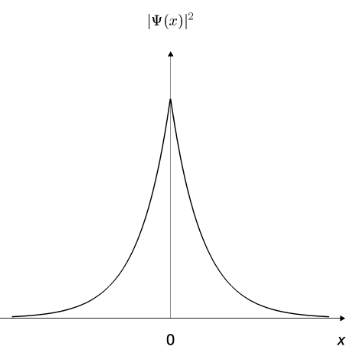
\includegraphics[width=0.25\linewidth]{image.png}
    \caption{Plot of $|\Psi (x,0)|^2$ over $x$}
    \label{fig:plot1}
\end{figure}
}
What's nice is that the probability of x being outside the range, is that it is 1 minus the probability it is \emph{within} the range. So we have:
\begin{equation}
    P([\braket{x} - \sigma, \braket{x} + \sigma]) = 1 - \int_{-\sigma}^{\sigma}\abs{\Psi(x,0)}^2\d x
\end{equation}
This integral:
\begin{equation}
    \int_{-\sigma}^{\sigma}\abs{\Psi(x,0)}^2\d x = \int_{-\sigma}^{\sigma} \lambda e^{-2\lambda \abs{x}}\d x
\end{equation}
From our earlier results we get:
\begin{equation}
    2\lambda \ab[\frac{1}{-2\lambda}e^{-2\lambda x}]\evalat_{0}^{\sigma} = -\ab[e^{-2\lambda \sigma} - 1] =1- e^{-2\lambda\sigma}
\end{equation}
We get for the argument:
\begin{equation}
    -2\lambda\sigma = -\frac{2\lambda\sqrt{2}}{2\lambda} = -\sqrt{2}
\end{equation}
This gives the probability as:
\begin{equation}
     \boxed{P([\braket{x} - \sigma, \braket{x} + \sigma]) = e^{-\sqrt{2}}\approx 0.24}
\end{equation}
\begin{figure}[H]
    \centering
    
\includegraphics[width=0.75\linewidth]{Q1F2.jpg}
    \caption{Filled in plot of figure \ref{fig:plot1}}
\end{figure}
\pagebreak